\documentclass{report}
\usepackage[colorlinks=true, linkcolor=blue]{hyperref}
\usepackage{graphicx}
\usepackage{subcaption}
\usepackage{amsmath}
\usepackage{float}
\usepackage[most]{tcolorbox}

\title{\Huge CS215 Assignment 1}
\author{Tamanna Kumari, 24B1015
\\\\Sagar V, 24B1021
\\\\Videep Reddy Jalapally, 24B1037}
\date{\today}

\begin{document}

\maketitle
\tableofcontents
\newpage

\section*{Question 1}
\addcontentsline{toc}{section}{Question 1}


\begin{tcolorbox}[colback=blue!5!white,colframe=blue!50!black,title=\textbf{Steps to Run}]
1. Open the provided q1.m Matlab file. \\
\\
2. The variable "f" at the beginning of the file sets the fraction of the data to corrupt. Set f = 0.3 for 30\% and f = 0.6 for 60\% and so on.\\
\\
3. Run the file in Matlab and it will print the Relative Mean Squared Errors in terminal and display the graphs shown below.
\end{tcolorbox}

\subsection*{$f = 30$}
\addcontentsline{toc}{subsection}{$f = 30$}

\begin{figure}[h]
    \centering
    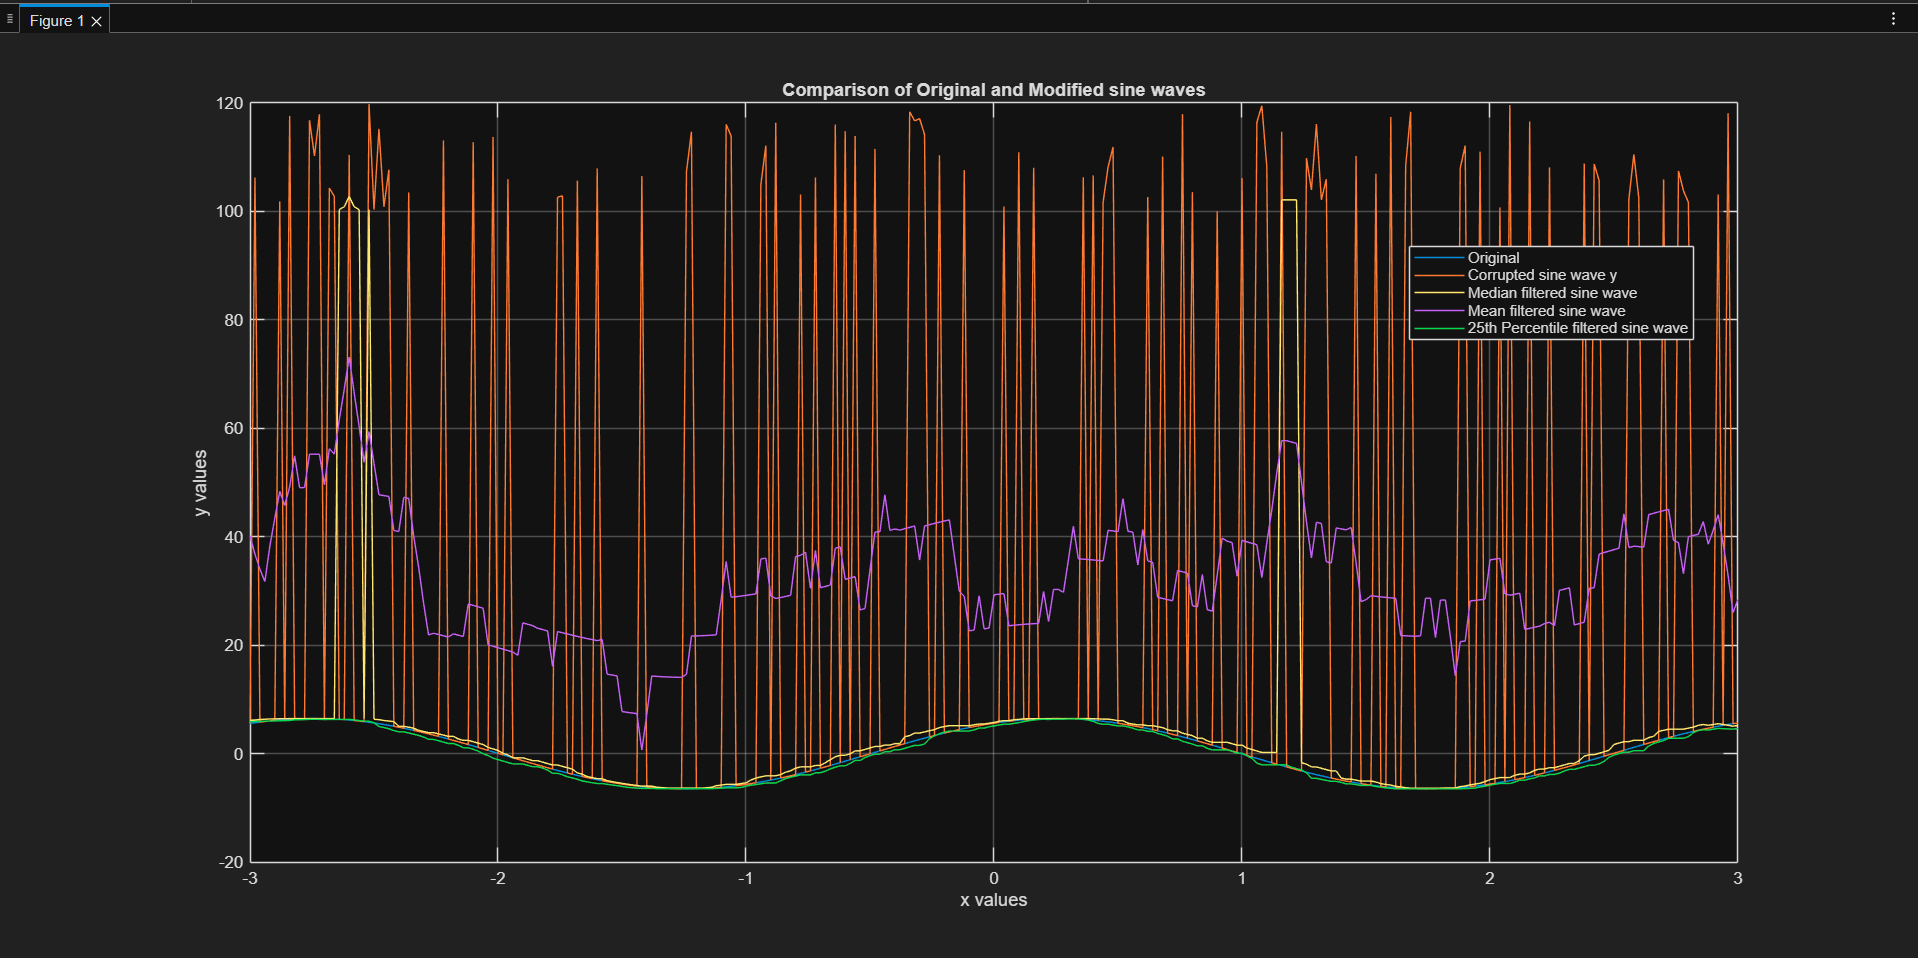
\includegraphics[width=0.9\textwidth]{f30_filtered.png}
    \caption{Graph plotted for $f = 30$.}
    \label{fig:f30}
\end{figure}

\vspace{1em} % space for adding explanation or notes
\noindent\textbf{Relative Mean Squared Error:}
\begin{align*}
\text{Median filtering: } 15.3467 \\
\text{Mean filtering: } 54.9060 \\
\text{25th percentile filtering: } 0.0131
\end{align*}\\


\begin{tcolorbox}[colback=green!5!white,colframe=green!50!black,title=\textbf{Observation from Graph and Relative Mean Errors}]
Observing the above graph and the relative mean errors, we can say that the \textbf{\textit{25th Percentile Filter}} filters it the best out of all the three filters, as the \textbf{relative mean squared error} for that filter is the \textbf{lowest}.  
The \textbf{\textit{Median Filter}} is a close second.  
The \textbf{\textit{Mean Filter}}, on the other hand, was \textbf{very far off} from the actual sine wave. This was consistent across multiple iterations of the code.
\end{tcolorbox}

\paragraph{} This is because the \textit{mean} is \textbf{drastically affected} by outliers in the dataset, as was the case here - the random values we added to “corrupt” the sine wave were in the range of \textit{100–120} (much higher than the range of the sine wave, $[-6.5, 6.5]$).

\paragraph{} The \textbf{\textit{Median Filter}} worked much better in this case, as it looks for the value closer to the \textbf{middle} of the dataset and hence is \textbf{less affected} by outliers or “spikes” in the data.

\paragraph{} The \textbf{\textit{25th Percentile Filter}} also performed \textbf{very well}, as it works similarly to the median filter but picks a value \textbf{lower} than the median — i.e., a value around the edge of the \textbf{first and second quartiles} in the ordered dataset. This makes it even more \textbf{immune} to outliers or “spikes” in the data which are in the higher end of the sorted data in the window.


\subsection*{\textbf{$f = 60$}}
\addcontentsline{toc}{subsection}{$f = 60$}

\begin{figure}[h]
    \centering
    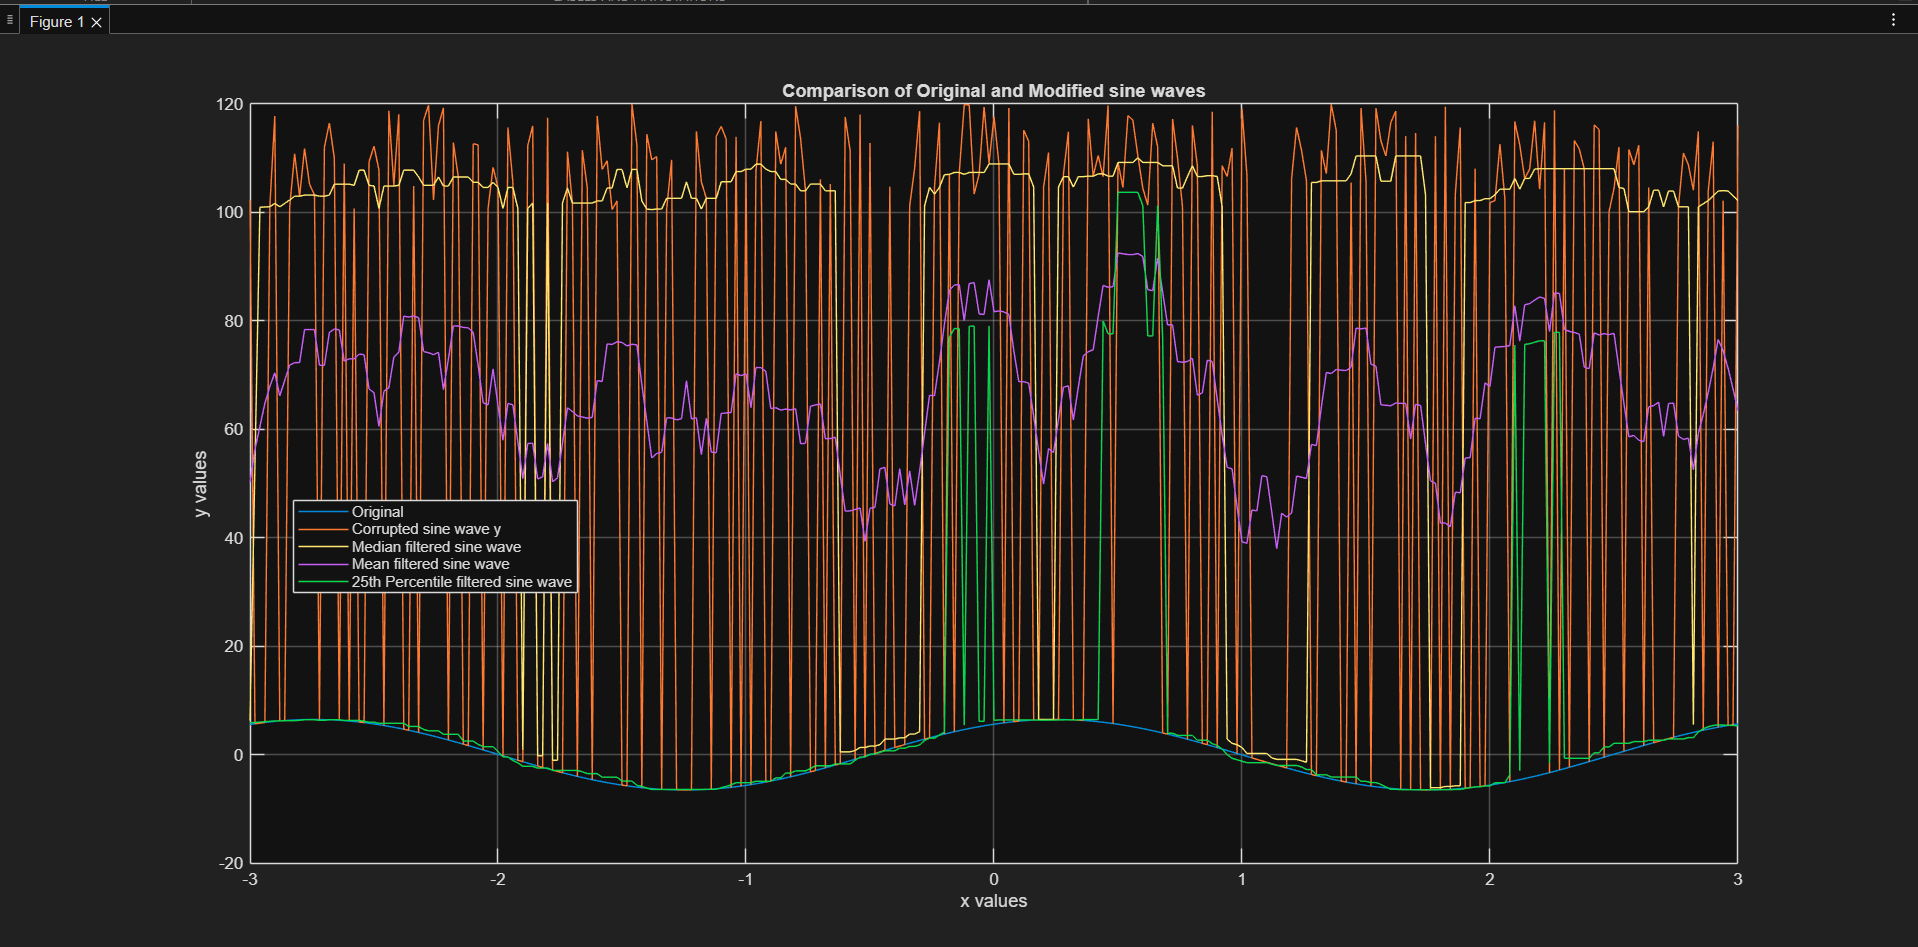
\includegraphics[width=0.9\textwidth]{f60_filtered.png}
    \caption{Graph plotted for $f = 60$.}
    \label{fig:f30}
\end{figure}


\vspace{1em} % space for adding explanation or notes
\noindent\textbf{Relative Mean Squared Error:}
\begin{align*}
\text{Median filtering: } 431.4391 \\
\text{Mean filtering: } 215.5709 \\
\text{25th percentile filtering: } 28.7075
\end{align*}\\

For \textit{f = 60}, the results change drastically.

\paragraph{} The \textbf{\textit{Mean Filter}}, as expected, still performed poorly. The filtering was not done well for the same reasons as above - it is \textbf{drastically affected} by outliers and for \textit{f = 60}, there were \textbf{double} the number of outliers as earlier. This result was consistent across multiple runs.

\paragraph{} The \textbf{\textit{Median Filter}}, on the other hand, resulted in a \textbf{much higher error} than the previous case. This can be attributed to the fact that there were \textbf{double} the number of “outliers” in this dataset compared to the first case. Due to this, the “middle” also shifts rapidly because, in every window, \textit{probabilistically speaking}, more than half the values are corrupted data. Hence, the filter is \textbf{very inaccurate}. This result was consistent across multiple runs.

\paragraph{} The \textbf{\textit{25th Percentile Filter}} is still the \textbf{best filter} out of all three. This is because it is much less affected by the “\textit{positive spikes}” - i.e., higher value outliers - as it looks for the border of the \textbf{first and second quartiles} in the ordered dataset. The higher values are less likely to affect this than the median or the mean filter.



\section*{Question 2}
\addcontentsline{toc}{section}{Question 2}
\subsection{Updating the Mean}

We want to compute the new mean after adding one new observation to an existing dataset, without recalculating from scratch.

\subsubsection*{Variable Definitions}
\begin{itemize}
    \item $n$: Number of observations in the dataset before the new value is added.
    \item $\bar{x}_{\text{old}}$: Mean of the dataset before adding the new value.
    \item $x_{\text{new}}$: The new observation being added to the dataset.
    \item $\bar{x}_{\text{new}}$: Mean of the dataset after adding the new value.
\end{itemize}

\subsubsection*{Derivation}
The old mean is given by:
\[
\bar{x}_{\text{old}} = \frac{1}{n} \sum_{i=1}^{n} x_i
\]
Multiplying through by $n$:
\[
\sum_{i=1}^{n} x_i = n \cdot \bar{x}_{\text{old}}
\]

After adding the new value $x_{\text{new}}$, the updated sum becomes:
\[
\sum_{i=1}^{n+1} x_i = \left( \sum_{i=1}^{n} x_i \right) + x_{\text{new}}
\]
\[
\sum_{i=1}^{n+1} x_i = n \cdot \bar{x}_{\text{old}} + x_{\text{new}}
\]

The new mean is:
\[
\bar{x}{\text{new}} = \frac{1}{n+1} \sum_{i=1}^{n+1} x_i
= \frac{n \cdot \bar{x}_{\text{old}} + x_{\text{new}}}{n+1}
\]

\subsubsection*{Final Formula}
\[
\boxed{\bar{x}_{\text{new}} = \frac{n \cdot \bar{x}_{\text{old}} + x_{\text{new}}}{n+1}}
\]

\subsubsection*{MATLAB Implementation}
\begin{verbatim}
function newMean = updateMean(oldMean, NewDataValue, n)
    newMean = (oldMean*n + NewDataValue)/(n+1);
end
\end{verbatim}

\subsection{Updating the Median}

\paragraph{Derivation and Explanation}  
The median of a dataset is defined as the value that has an equal number of elements greater than it and less than it.  

We consider two cases depending on whether the original array length $n$ is even or odd.  

\subsubsection*{Case 1: $n$ even}  
If the current array has an even number of elements $n$, the median lies between $A_{\frac{n}{2}}$ and $A_{\frac{n}{2} + 1}$.  


When a new value $x$ is added, the total size becomes $n+1$ (odd), so the median will be the single middle element. The possibilities are:\\  


- If $x < A_{\frac{n}{2}}$:  
  $A_{\frac{n}{2}}$ now has $\frac{n}{2}$ elements less than it (the previous $\frac{n}{2} - 1$ plus the new $x$) and $\frac{n}{2}$ elements greater than it. Hence $A_{\frac{n}{2}}$ becomes the median.\\


- If $A_{\frac{n}{2}} \leq x \leq A_{\frac{n}{2} + 1}$:  
  $x$ has $\frac{n}{2}$ elements less than it and $\frac{n}{2}$ greater than it, so $x$ becomes the median.\\
  

- If $x > A_{\frac{n}{2} + 1}$:  
  $A_{\frac{n}{2} + 1}$ now has $\frac{n}{2}$ elements less than it and $\frac{n}{2}$ greater than it (the previous $\frac{n}{2} - 1$ plus $x$). Thus $A_{\frac{n}{2} + 1}$ becomes the median.
  

\subsubsection*{Case 2: $n$ odd}  
If the original array length $n$ is odd, the median is $A_{\frac{n+1}{2}}$. After adding a new element, the size becomes even ($n+1$), so the median will be the average of the two middlemost elements.

Let:
\[
m = \frac{n+1}{2} \quad index \quad of \quad old \quad median
\]
and note that before insertion:
- $A_m$ has $\frac{n-1}{2}$ elements less than it
- $A_m$ has $\frac{n-1}{2}$ elements greater than it

After insertion:

- If $x < A_{m-1}$:  
  The two middlemost elements become $A_{m-1}$ and $A_m$. Each has an equal number of lesser and greater elements, so the median is:
  \[
  \frac{A_{m-1} + A_m}{2}
  \]

- If $A_{m-1} \leq x \leq A_{m+1}$:  
  The middle two elements are $A_m$ and $x$, which have equal counts of lesser and greater elements. The median is:
  \[
  \frac{A_m + x}{2}
  \]

- If $x > A_{m+1}$:  
  The middle two elements are $A_m$ and $A_{m+1}$, giving:
  \[
  \frac{A_m + A_{m+1}}{2}
  \]

\begin{verbatim}
function newMedian = updateMedian(OldMedian, NewDataValue, A, n)

    if mod(n,2) == 0
        if NewDataValue > A(n/2 + 1)
            newMedian = A(n/2 + 1);
        elseif NewDataValue < A(n/2)
            newMedian = A(n/2);
        else
            newMedian = NewDataValue;
        end
    else
        if NewDataValue < A((n-1)/2)
            newMedian = (A((n-1)/2) + A((n+1)/2)) /2;
        elseif NewDataValue < A((n+1)/2 + 1)
            newMedian = (OldMedian + NewDataValue)/2;
        else
            newMedian = (A((n+1)/2) + A((n+3)/2))/2;
        end
    end
end
\end{verbatim}

\subsection{Updating Standard Deviation}

\paragraph{Setup.}
Let the old dataset be $x_1,\dots,x_n$ with sample mean $\bar{x_{old    }}$ and sample standard deviation $s_{old}$:\\

\[
\begin{aligned}
s_{\text{old}}^{2} 
&= \frac{\sum_{i=1}^{n} (x_i - \bar{x}_{\text{old}})^2}{n-1} \\[6pt]
&= \frac{\sum_{i=1}^{n} \left(x_i^2 - 2x_i\bar{x}_{\text{old}} + \bar{x}_{\text{old}}^{\,2}\right)}{n-1} \\[6pt]
&= \frac{\sum_{i=1}^{n} x_i^2 - 2\bar{x}_{\text{old}} \sum_{i=1}^{n} x_i + \sum_{i=1}^{n} \bar{x}_{\text{old}}^{\,2}}{n-1} \\[6pt]
&= \frac{\sum_{i=1}^{n} x_i^2 - 2\bar{x}_{\text{old}} \cdot (n\bar{x}_{\text{old}}) + n\bar{x}_{\text{old}}^{\,2}}{n-1} \\[6pt]
&= \frac{\sum_{i=1}^{n} x_i^2 - 2n\bar{x}_{\text{old}}^{\,2} + n\bar{x}_{\text{old}}^{\,2}}{n-1} \\[6pt]
&= \frac{\sum_{i=1}^{n} x_i^2 - n\bar{x}_{\text{old}}^{\,2}}{n-1}.
\end{aligned}
\]

A new observation $x_{\text{new}}$ arrives. Let the updated sample size be $n+1$, the updated mean be $\bar{x}_{\text{new}}$, and the updated sample standard deviation be $s_{\text{new}}$.

\paragraph{Key identities.}
From the old sample variance formula,
\[
\sum_{i=1}^{n} x_i^2 \;=\; (n-1)\,s_{\text{old}}^2 \;+\; n\,\bar{x}_{\text{old}}^{\,2}.
\]
After adding $x_{\text{new}}$,
\[
\sum_{i=1}^{n+1} x_i^2 \;=\; \Big(\sum_{i=1}^{n} x_i^2\Big) \;+\; x_{\text{new}}^{\,2}
\;=\; (n-1)\,s_{\text{old}}^2 \;+\; n\,\bar{x}_{\text{old}}^{\,2} \;+\; x_{\text{new}}^{\,2}.
\]

\paragraph{Updated variance (sample).}
By the computational form for the new sample variance with $n+1$ samples (denominator $(n+1)-1=n$),
\[
s_{\text{new}}^{\,2}
\;=\;
\frac{\displaystyle \sum_{i=1}^{n+1} x_i^2 \;-\; (n+1)\,\bar{x}_{\text{new}}^{\,2}}{n}
\;=\;
\frac{(n-1)\,s_{\text{old}}^2 \;+\; n\,\bar{x}_{\text{old}}^{\,2} \;+\; x_{\text{new}}^{\,2} \;-\; (n+1)\,\bar{x}_{\text{new}}^{\,2}}{n}.
\]

\paragraph{Final formula.}
\[
\boxed{\;
s_{\text{new}}
\;=\;
\sqrt{\frac{(n-1)\,s_{\text{old}}^2 \;+\; n\,\bar{x}_{\text{old}}^{\,2} \;+\; x_{\text{new}}^{\,2} \;-\; (n+1)\,\bar{x}_{\text{new}}^{\,2}}{n}}
\; }.
\]

\noindent\textbf{MATLAB Implementation}
\begin{verbatim}
function newStd = UpdateStd(OldMean, OldStd, NewMean, NewDataValue, n)
    newStd = sqrt(((OldStd^2) * (n-1) + NewDataValue^2 + n * (OldMean^2) - (n+1)*(NewMean^2))/n);
end
\end{verbatim}

\subsection{Incremental Histogram Update}

When adding a new observation $x_{\text{new}}$ to an existing histogram, a full recomputation is unnecessary.  
Let the histogram have bins $B_1, B_2, \dots, B_k$ with counts $h_1, h_2, \dots, h_k$.  
Determine the bin index
\[
j \;=\; \operatorname{argmin}{m} \ \{\, x_{\text{new}} \in B_m \,\}.
\]
Increment the corresponding bin height:
\[
h_j \;\leftarrow\; h_j + 1.
\]
All other bin heights remain unchanged:
\[
h_m \ \text{unchanged for} \ m \neq j.
\]

\section*{Question 3}
\addcontentsline{toc}{section}{Question 3}
Bonferroni's inequality states that for two events \( A \) and \( B \):

\[P(A \cap B) \geq P(A) + P(B) - 1 \]

We know that \( P(A) \geq 1 - q_1 \) and \( P(B) \geq 1 - q_2\).
Thus, we can write:
\[P(A \cap B) \geq (1 - q_1) + (1 - q_2) - 1\]
\[P(A \cap B) \geq 1 - (q_1 + q_2)\]
Hence, proven that \( P(A \cap B) \geq 1 - (q_1 + q_2) \).

\section*{Question 4}
\addcontentsline{toc}{section}{Question 4}

Labelling events: \\
 \begin{description}
\item[R]Event that a bus in town is red.
\item[B] Event that a bus in town in blue.
\item[SR] Event that the person sees red.
 \end{description}

Given: 

\[P(R) = 0.01\] 
\[P(B) = 0.99\] 
\[P(SR | R) = 0.99\]
\[P (SR | B) = 0.02\]

To find: 
\[P ( R | SR )\]

Soln :
\[P ( R | SR) = \frac{P ( SR | R ) \cdot P ( R )}{P ( SR )}\]
Using the law of total probability, we can express \( P(SR) \):
\[P(SR) = P(SR | R) \cdot P(R) + P(SR | B) \cdot P(B)\]
Substituting the values:
\[P(SR) = 0.99 \cdot 0.01 + 0.02 \cdot 0.99\]
\[P(SR) = 0.0099 + 0.0198 = 0.0297\]
Now substituting back into the equation for \( P(R | SR) \):
\[P(R | SR) = \frac{0.99 \cdot 0.01}{0.0297}\]
\[P(R | SR) = \frac{0.0099}{0.0297}\]
\[P(R | SR) \approx 0.3333\]        

Thus, the probability that the bus is red given that the person sees red is approximately \( 0.3333 \).

\section*{Question 5}
\addcontentsline{toc}{section}{Question 5}
Events:
\begin{description}
    \item[A] Event that a voter prefers A.
    \item[B] Event that a voter prefers B.
    \item[Wi] Event that exactly i out of 3 people prefer A.
\end{description}

Given:
\[P(A) = 0.95\]
\[P(B) = 0.05\]

Let's say i out of the three people preferred A in the poll and the rest preferred B.

Ways to choose i people from 3:
\begin{equation}
\binom{3}{i} = \frac{3!}{i!(3-i)!}
\label{eq:binomial}
\end{equation}

The probability of choosing i people who prefer A and 3-i people who prefer B is given by:
\[ P(Wi) = \binom{3}{i} \cdot (0.95)^i \cdot (0.05)^{3-i}\]  

Values of i can be 0, 1, 2, or 3.
The probability that the exit poll declared majority of A is given by:
\[P(W2) + P(W3)\]
Calculating \( P(W2) \):
\[P(W2) = \binom{3}{2} \cdot (0.95)^2 \cdot (0.05)^1\]
\[= 3 \cdot (0.95)^2 \cdot (0.05)\]
\[= 3 \cdot 0.9025 \cdot 0.05\]
\[= 3 \cdot 0.045125\]
\[= 0.135375\]      

Calculating \( P(W3) \):
\[P(W3) = \binom{3}{3} \cdot (0.95)^3 \cdot (0.05)^0\]
\[= 1 \cdot (0.95)^3 \cdot 1\]
\[= (0. 95)^3\]
\[= 0.857375\]
Thus, the total probability that the exit poll declared majority of A is:
\[P(W2) + P(W3) = 0.135375 + 0.857375\]
\[= 0.99275\]

\vspace{1em}

\noindent
Even with \textbf{10,000 residents}, since \textbf{95\%} of the people prefer \textbf{candidate A} over \textbf{candidate B}, the probabilities remain the same:
\[
P(A) = 0.95, \qquad P(B) = 0.05
\]

\noindent
Since these probabilities are \textit{unchanged}, there will be \textbf{no difference} in our calculation for the accuracy of the exit poll. Therefore, the accuracy still equals:
\[
\text{Accuracy} = \mathbf{0.99275}
\]


\section*{Question 6}
\addcontentsline{toc}{section}{Question 6}

Number of people in the town = \( m \) \\
Number of people in the subset = \( n \) \\
Probability that a person prefers A = \( p \) \\
\[
q(\mathcal{S}) = \frac{\sum_{i \in I(\mathcal{S})} x_i}{n}
\]
where \( I(\mathcal{S}) \) is a set containing the index (from \(1\) to \(m\)) of each voter in \(\mathcal{S}\) and \(x_i = 1\) iff \( i^{th}\) person prefers A.
\\ \\
Total number of subsets of size \( n \) from \( m \) = \(m ^ n\)\\\\
Number of subsets of size \(n\) such that i number of people out of them prefer A = \[ m^n \sum_{i=0}^{n} (1-p) ^{n - i} (p)^i\binom{n}{i} \]

\(q(\mathcal{S})\) for each such subset where i people prefer A is 
\[q(\mathcal{S}) = \frac{i}{n}\]
 Thus \(q(\mathcal{S})\) for all such subset where i people prefer A is 
\[m^n \sum_{i=0}^{n} \frac{i}{n} \cdot \binom{n}{i}(1-p) ^{n - i} (p)^i\] 

\subsection*{(a)}
To show:
\[
\sum_\mathcal{S} \frac{q(\mathcal{S})}{m^{n}} = p.
\]

Soln:

Consider the binomial equation
\[(xp + (1-p))^n = \sum_{i=0}^{n}\binom{n}{i}(1-p) ^{n - i} (x)^i(p)^i\]
Differentiating both sides with respect to \(x\):
\\LHS : 
\[\frac{d}{dx}((xp + (1-p))^n) = n(xp + (1-p))^{n-1}p\]
\\RHS:
\[\frac{d}{dx}(\sum_{i=0}^{n}\binom{n}{i}(1-p)^{n-i}x^i p^i) = \sum_{i=0}^{n} i \cdot \binom{n}{i}(1-p)^{n-i}x^{i-1}p^i\]
Substituting \(x = 1\):
\\LHS:
\[n(p + (1-p))^{n-1}p = n \cdot p\]
\\RHS:
\[\sum_{i=0}^{n} i \cdot \binom{n}{i}(1-p)^{n-i}p^i\]
Thus, we have:
\begin{equation}
\sum_{i=0}^{n} i \cdot \binom{n}{i}(1-p)^{n-i}p^i = n \cdot p
\label{eq:binomial_diff}
\end{equation}
Dividing both sides by \(n\):

\[\sum_{i=0}^{n} \frac{i}{n} \cdot \binom{n}{i}(1-p)^{n-i}p^i = p\]
Now, multiplying both sides by \(m^n\):
\[m^n \sum_{i=0}^{n} \frac{i}{n} \cdot \binom{n}{i}(1-p)^{n-i}p^i = m^n \cdot p\]
Thus, we have:
\[\sum_\mathcal{S} \frac{q(\mathcal{S})}{m^{n}} = p\]

\subsection*{(b)}
To show:
\[
    \sum_{S} \frac{q^{2}(\mathcal{S})}{m^{n}} = \frac{p}{n} + \frac{p^{2}(n-1)}{n}.
\]
Soln:
    \(q^2(\mathcal{S})\) for each such subset where i people prefer A is 
    \[q^2(\mathcal{S}) = (\frac{i}{n})^2\]
    Thus \(q^2(\mathcal{S})\) for all such subset where i people prefer A is
    \[m^n \sum_{i=0}^{n} \frac{i^2}{n^2} \cdot \binom{n}{i}(1-p)^{n - i} (p)^i\]
    Using the binomial equation:
    \[(xp + (1-p))^n = \sum_{i=0}^{n}\binom{n}{i}(1-p)^{n-i}x^i p^i\]
    Differentiating twice with respect to \(x\):
    \\LHS:
    \[\frac{d^2}{dx^2}((xp + (1-p))^n) = n(n-1)(xp + (1-p))^{n-2}p^2 \]
    \\RHS: 
    \[\frac{d^2}{dx^2}(\sum_{i=0}^{n}\binom{n}{i}(1-p)^{n-i}x^i p^i) = \sum_{i=0}^{n} i(i-1) \cdot \binom{n}{i}(1-p)^{n-i}x^{i-2}p^i\]
    Substituting \(x = 1\):
    \\LHS:
    \[n(n-1)(p + (1-p))^{n-2}p^2 = n(n-1)p^2\]
    \\RHS:  
    \[\sum_{i=0}^{n} i(i-1) \cdot \binom{n}{i}(1-p)^{n-i}p^i\]
    Thus, we have:
    \[\sum_{i=0}^{n} i(i-1) \cdot \binom{n}{i}(1-p)^{n-i}p^i = n(n-1)p^2\]
    \[\sum_{i=0}^{n} i^2 \cdot \binom{n}{i}(1-p)^{n-i}p^i - \sum_{i=0}^{n} i \cdot \binom{n}{i}(1-p)^{n-i}p^i = n(n-1)p^2\]
    Using {\ref{eq:binomial_diff}}:
    \[\sum_{i=0}^{n} i^2 \cdot \binom{n}{i}(1-p)^{n-i}p^i -np = n(n-1)p^2\]
    Dividing both sides by \(n^2\) and nultiplying by \(m^n\):
    \[m^n \sum_{i=0}^{n} \frac{i^2}{n^2} \cdot \binom{n}{i}(1-p)^{n-i}p^i - m^n \cdot \frac{p}{n} = m^n \cdot \frac{(n-1)p^2}{n}\]
    Thus, we have:
    \[\sum_{S} \frac{q^{2}(\mathcal{S})}{m^{n}} = \frac{p}{n} + \frac{p^{2}(n-1)}{n}\]

\subsection*{(c)}
To show:
\[
    \sum_{S} \frac{\left(q(S) - p\right)^{2}}{m^{n}} = \frac{p(1-p)}{n}.
\]

Soln:
We can rewrite the left-hand side as:
\[\sum_{S} \frac{q^2(\mathcal{S})}{m^{n}} + \sum_{S} \frac{p^{  2}}{m^{n}} - 2p\sum_{S} \frac{q(\mathcal{S})}{m^{n}}\]
Substituting the value of \(\sum_{S} \frac{q(\mathcal{S})}{m^{n}} = p\):
\[\sum_{S} \frac{q^2(\mathcal{S})}{m^{n}} + \sum_{S} \frac{p^{  2}}{m^{n}} - 2p^{2}\]
Now substituting the value of \(\sum_{S} \frac{q^2(\mathcal{S})}{m^{n}} = \frac{p}{n} + \frac{p^{2}(n-1)}{n}\):
\[\frac{p}{n} + \frac{p^{2}(n-1)}{n} - 2p^{2} + m^{n}\frac{p^{  2}}{m^{n}}\]
Hence

\[\sum_{S} \frac{\left(q(S) - p\right)^{2}}{m^{n}} = \frac{p^2n + p -p^2}{n} - p^2\]
Thus, we have shown that:
\[\sum_{S} \frac{\left(q(S) - p\right)^{2}}{m^{n}} = \frac{p(1-p)}{n}\]

\subsection*{(d)}
\(q_i(\mathcal{S})\) : \(q(\mathcal{S})\) for \(i^{th}\) subset of n elements.
\\\\
There are \(m^n\) subsets of size \(n\) from \(m\) people.
\\\\
Let 
\[S_k = \{q(\mathcal{S})  : |q(S)-p| > \delta \}\]

Consider $\sigma$ as the standard deviation of \(q(\mathcal{S})\):

\[\sigma = \sqrt{\sum_{\mathcal{S}} \frac{(q_i(\mathcal{S}) - p)^{2}}{m^{n}-1}}\]
We can write 
\[\delta = \delta \cdot \frac{\sigma}{\sigma}\]
Let \(\frac{\delta}{\sigma} = k\) Clealry \( k >  0\). So,
\[S_k = \{q(\mathcal{S})  : |q(S)-p| > k\sigma \}\]
Using Two-sided Chebyshev's inequality:

\[\frac{|S_k|}{m^n}  \leq  \frac{1}{k^2}\]

\[\implies \frac{|S_k|}{m^n}  \leq  \frac{\sigma ^ 2}{\delta^2}\]
\[\implies \frac{|S_k|}{m^n}  \leq  \frac{({\sum_{\mathcal{S}} \frac{(q_i(\mathcal{S}) - p)^{2}}{m^{n}-1}}) }{\delta^2}\]

Now,
\[\sum_{\mathcal{S}} \frac{(q_i(\mathcal{S}) - p)^{2}}{m^{n}-1} = \sum_{\mathcal{S}} \frac{\left(q(S) - p\right)^{2}}{m^{n}} \cdot {\frac{m^n}{m^n -1}}\]
Using the result from part (c):
\[\sum_{\mathcal{S}} \frac{(q_i(\mathcal{S}) - p)^{2}}{m^{n}-1} =\frac{p(1-p)}{n} \cdot {\frac{m^n}{m^n -1}} \leq {\frac{p(1-p)}{n}}\]

So,
\[\frac{|S_k|}{m^n}  \leq  \frac{({\sum_{\mathcal{S}} \frac{(q_i(\mathcal{S}) - p)^{2}}{m^{n}-1}}) }{\delta^2}\leq {\frac{p(1-p)}{n}} \cdot \frac{1}{\delta^2}\]\\

This is a very nice application of Chebychev's inequality.
Significance of this result is that it gives us a bound on the fraction of subsets whose average preference deviates from the true preference by more than a certain amount, \(\delta\).
We notice that this proportion is quite small which means we can be confident that most subsets will have an average preference pretty close to the true preference \(p\).

\end{document}
